% Created 2013-01-20 Sun 14:37
\documentclass[bigger]{beamer}
      \mode<presentation>
      \usetheme{Darmstadt}
      \setbeamercovered{{{{transparent}}}}
      \usecolortheme{lily}
      \usepackage[spanish]{babel}
%%      \beamertemplateballitem
%%      \setbeameroption{show notes}
      \usepackage[utf8]{inputenc}
      \usepackage[T1]{fontenc}
      \usepackage{hyperref}
      \usepackage{color}
      \usepackage{listings}
      \usepackage{alltt}
      \usepackage{verbatim}
      \usepackage{hyperref}
      \usepackage{array}
      %% ulem nos da mayor control de subrayados, \normalem evita que todos
      %% los \em sean subrayados
      \usepackage{ulem}
      \normalem
%%      \lstset{numbers=none,language=[ISO]C++,tabsize=4,
%%  frame=single,
%%  basicstyle=\small,
%%  showspaces=false,showstringspaces=false,
%%  showtabs=false,
%%  keywordstyle=\color{blue}\bfseries,
%%  commentstyle=\color{red},
%%  }

    \newcommand{\confurl}{\url{{{{beamerconfurl}}}}}

      \institute{Facultad de Ingeniería, UNAM}
       \subject{{{{beamersubject}}}}
\usepackage[utf8]{inputenc}
\usepackage[T1]{fontenc}
\usepackage{fixltx2e}
\usepackage{graphicx}
\usepackage{longtable}
\usepackage{float}
\usepackage{wrapfig}
\usepackage{soul}
\usepackage{t1enc}
\usepackage{textcomp}
\usepackage{marvosym}
\usepackage{wasysym}
\usepackage{latexsym}
\usepackage{amssymb}
\usepackage{hyperref}
\tolerance=1000
\usepackage{color}
\usepackage{listings}
\providecommand{\alert}[1]{\textbf{#1}}

\title{Sistemas Operativos:\\Presentación del curso}
\author{Gunnar Wolf}
\date{20 January 2013}

\pgfdeclareimage[height=1.5cm]{../img/pres/cintillo.png}{../img/pres/cintillo.png}\logo{\pgfuseimage{../img/pres/cintillo.png}}
\AtBeginSection[]{ \begin{frame}<beamer> \frametitle{Índice} \tableofcontents[currentsection] \end{frame} }
\begin{document}

\maketitle


\section{Punto de partida}
\label{sec-1}
\begin{frame}[fragile]\frametitle{Mis coordenadas}
\label{sec-1_1}

\begin{center}
Personales
\end{center}

\begin{description}
\item[Nombre] Gunnar Eyal Wolf Iszaevich
\item[E-mail] gwolf+sistop@gwolf.org
\item[Ubicación] Instituto de Investigaciones Económicas UNAM
\end{description}


\begin{center}
Del curso
\end{center}

\begin{description}
\item[Página Web] \href{http://sistop.gwolf.org/}{http://sistop.gwolf.org/}
\end{description}
\end{frame}
\begin{frame}[fragile]\frametitle{Horario, calendario}
\label{sec-1_2}

\begin{itemize}
\item Lunes, miércoles y viernes
\item 13:00 a 14:30
\item Salón ***
\item 72 horas clase en total… En teoría.

\begin{itemize}
\item Feriados 4 de febrero, 18 de marzo, 1, 10 y 15 de mayo
\item Una sesión de presentación; estimo tres exámenes parciales
\end{itemize}

\item La realidad: 52.5 horas efectivas de clase.
\end{itemize}
\end{frame}
\section{Encuadre del curso}
\label{sec-2}
\begin{frame}[fragile]\frametitle{El curso dentro de la currícula de la carrera}
\label{sec-2_1}

\begin{center}
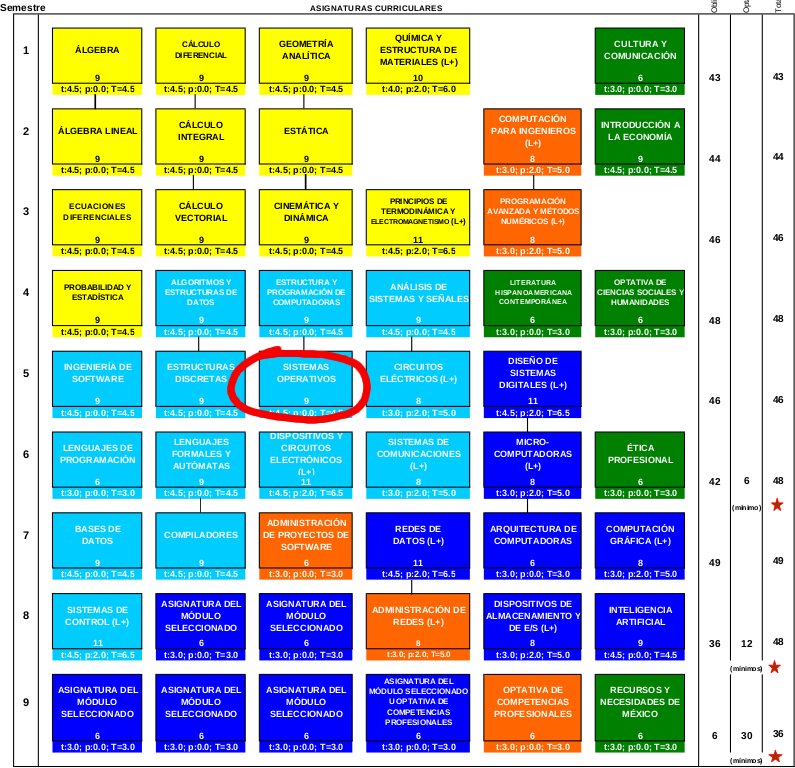
\includegraphics[width=0.7\textwidth]{../img/pres/mapa_curricular.png}
\end{center}
\end{frame}
\begin{frame}[fragile]\frametitle{Seriación y materias relacionadas}
\label{sec-2_2}

\begin{itemize}
\item Seriación obligatoria: \emph{Estructura y programación de computadoras}
\item Asumo familiaridad con:

\begin{itemize}
\item Computación para ingenieros
\item Programación avanzada y métodos numéricos
\item Algoritmos y estructura de datos
\end{itemize}

\end{itemize}
\end{frame}
\begin{frame}[fragile]\frametitle{Lenguajes de programación}
\label{sec-2_3}

\begin{itemize}
\item Familiaridad con algún lenguaje de programación de alto nivel

\begin{itemize}
\item Para seguir ejemplos (que serán principalmente en shell POSIX,
    Ruby, Perl y Python)
\item Para hacer ejercicios en clase (basta con pseudocódigo
    semi-formal)
\item Para tareas (¡código legal/válido!)
\end{itemize}

\item Familiaridad básica con C

\begin{itemize}
\item Más para leer que para desarrollar
\end{itemize}

\end{itemize}
\end{frame}
\begin{frame}[fragile]\frametitle{Otros requisitos}
\label{sec-2_4}

\begin{center}
Linux (GNU) / Unix
\end{center}

\begin{itemize}
\item \textbf{Muy} conveniente tener acceso a un sistema basado en Linux, o algún
  Unix
\item \textbf{Muy} preferentemente, software libre
\end{itemize}


\begin{center}
Lectura en inglés
\begin{itemize}
\item Buena parte del material de referencia es en inglés
\item El material de estudios de caso casi siempre es en inglés
\item Nivel de comprensión de lectura \textbf{muy} recomendado
\end{itemize}
\end{frame}
\begin{frame}[fragile]\frametitle{Programa de estudio}
\label{sec-2_5}

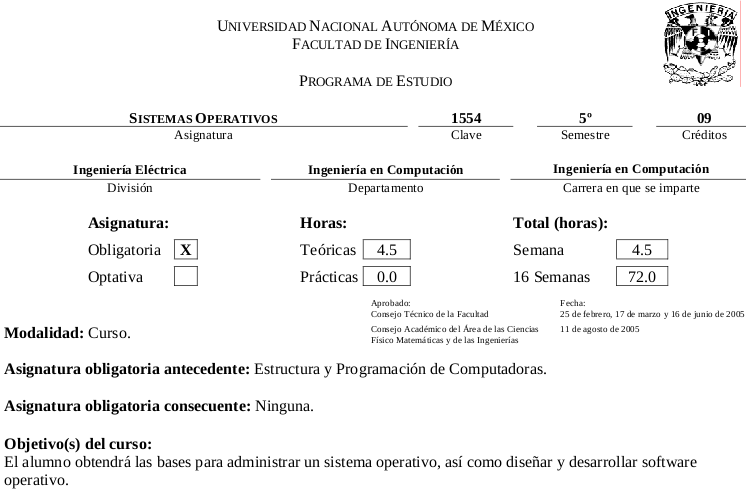
\includegraphics[width=\textwidth]{../img/pres/prog_estudio.png}
\end{center}
\end{frame}
\section{Enfoque personal}
\label{sec-3}
\begin{frame}[fragile]\frametitle{¿Quién soy y por qué estoy aquí?}
\label{sec-3_1}

\begin{itemize}
\item Formación autodidacta

\begin{itemize}
\item La necesidad es el mejor motor para aprender algo
\item ¿No conocemos algo que necesitamos? Lo aprendemos sobre la marcha
\item ¿Aprender algo para lo que no tengo uso? Aprendizaje destinado al
    olvido/fracaso
\end{itemize}

\item Usuario, promotor y desarrollador de software libre
\end{itemize}
\end{frame}
\begin{frame}[fragile]\frametitle{¿Por qué me parece importante la materia?}
\label{sec-3_2}

\begin{itemize}
\item No espero que se dediquen a \emph{escribir} sistemas operativos (aunque
  puede ocurrir)
\item Pero en cualquier área de aplicación profesional \emph{requerimos conocer   su funcionamiento} para desempeñarnos mejor

\begin{itemize}
\item Citando el objetivo institucional de la materia, \emph{administrar un     sistema operativo} y \emph{diseñar y desarrollar software operativo}
\end{itemize}

\item Lo que veamos en esta materia tendrá aplicación prácticamente en
  cualquier área de desempeño profesional
\end{itemize}
\end{frame}
\begin{frame}[fragile]\frametitle{¿Qué debemos lograr?}
\label{sec-3_3}

\begin{center}
La Facultad dice que:\\
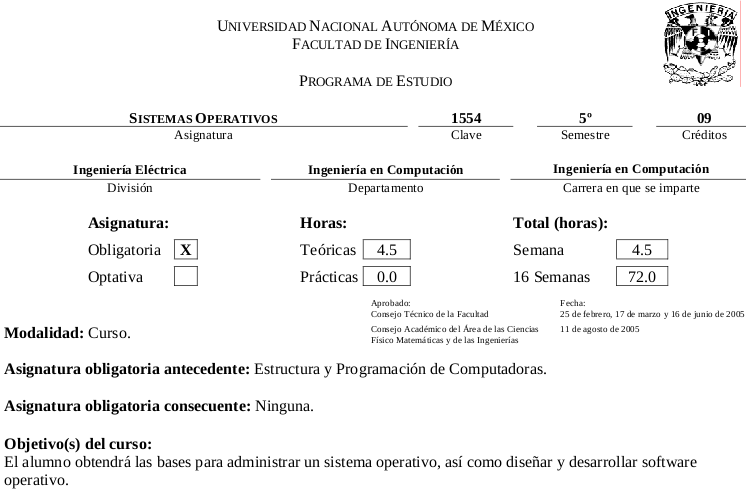
\includegraphics[width=0.9\textwidth]{../img/pres/prog_estudio.png}
\end{center}
\end{frame}
\begin{frame}[fragile]\frametitle{¿Qué espero que logremos?}
\label{sec-3_4}

\begin{itemize}
\item Comprender la función de
\end{itemize}
\end{frame}
\section{Estructura del curso}
\label{sec-4}
\begin{frame}[fragile]\frametitle{Unidades}
\label{sec-4_1}

\begin{enumerate}
\item Introducción a los sistemas operativos
\item Administración de procesos
\item Administración de memoria
\item Planificación de procesos
\item Sistemas de archivos
\item Sistemas de entrada/salida
\item Sistemas distribuidos
\item Seguridad y medidas de desempeño
\end{enumerate}
\end{frame}
\section{Forma de evaluación}
\label{sec-5}
\begin{frame}[fragile]\frametitle{Porcentajes de evaluación}
\label{sec-5_1}
\end{frame}
\begin{frame}[fragile]\frametitle{Toma de asistencia}
\label{sec-5_2}
\end{frame}
\section{Bibliografía}
\label{sec-6}
\begin{frame}[fragile]\frametitle{Bibliografía oficial del curso}
\label{sec-6_1}

\vfill {\scriptsize
\begin{columns}\begin{column}{0.4\textwidth}
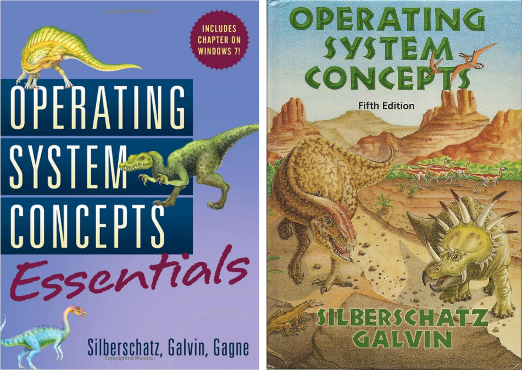
\includegraphics[height=10em]{../img/pres/libro_silberschatz.png}
\vskip 2em
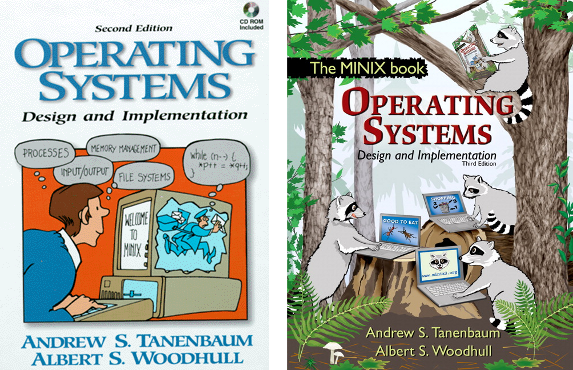
\includegraphics[height=10em]{../img/pres/libro_tanenbaum.png}
\end{column}\begin{column}{0.5\textwidth}
{\large Operating System Concept Essentials} \\
Abraham Silberschatz, Peter Baen Galvin, Greg Gagne\\
Wiley (Traducción: Limusa)\\
5ª edición (1998) en adelante
\vskip 2em
{\large Sistemas operativos: Diseño e implementación} \\
Andrew S. Tanenbaum y Albert S. Woodhull \\
Prentice Hall\\
2ª (1997) o 3ª (2006) ediciones
\end{column}\end{columns}
\end{frame}
\begin{frame}[fragile]\frametitle{Libros descargables disponibles en español}
\label{sec-6_2}

\vfill {\scriptsize
\begin{columns}\begin{column}{0.25\textwidth} \vskip 10em
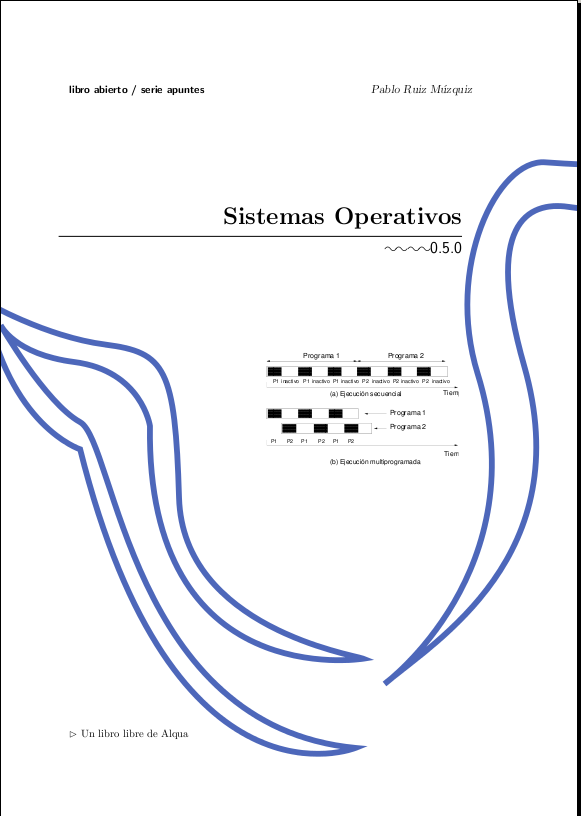
\includegraphics[height=10em]{../img/pres/libro_ruiz.png}
\end{column}\begin{column}{0.7\textwidth}
{\large Sistemas Operativos} \\
Luis La Red Martínez\\ Universidad Nacional del Nordeste (Argentina)\\
\href{http://exa.unne.edu.ar/depar/areas/informatica/SistemasOperativos/sistope2.PDF}{Disponible en línea} desde \href{http://exa.unne.edu.ar/depar/areas/informatica/SistemasOperativos/SOF.htm}{el sitio Web del autor} (y también con \href{http://sistop.gwolf.org/biblio/Sistemas_Operativos_-_Luis_La_Red_Martinez.pdf}{copia local} en la página del curso)
\vskip 2em {\large Sistemas operativos} \\
Pablo Ruiz Múzquiz\\
Libro Abierto / Serie Apuntes, 2004\\
\href{http://forja.rediris.es/frs/download.php/1922/SSOO-0_5_0.pdf}{Disponible en línea} desde la \href{http://alqua.tiddlyspace.com/}{editorial de textos libres Alqua} (y
también con \href{http://sistop.gwolf.org/biblio/Sistemas_Operativos_-_Pablo_Ruiz_Muzquiz.pdf}{copia local} en la página del curso)
\end{column}\end{columns}
\end{frame}
\begin{frame}[fragile]\frametitle{Otros textos recomendados}
\label{sec-6_3}


{\large An operating systems vade mecum } \\
Raphael Finkel\\
University of Kentucky - Lexington, 1988\\
\href{ftp://ftp.cs.uky.edu/cs/manuscripts/vade.mecum.2.pdf}{Disponible en línea} desde \href{http://www.cs.uky.edu/~raphael/}{el sitio Web del autor} (y también con \href{http://sistop.gwolf.org/biblio/An_operating_system_vade_mecum_-_Raphael_Finkel.pdf}{copia local} en la página del curso)

\vskip 2em {\large A short introduction to operating systems } \\
Mark Burgess\\
Oslo University College, 2001 \\
\href{http://www.iu.hio.no/~mark/os/os.pdf}{Disponible en línea} desde \href{http://cfengine.com/markburgess/writing.html}{el sitio Web del autor} (y también
con \href{http://sistop.gwolf.org/biblio/Short_introduction_to_operating_systems_-_Mark_Burgess.pdf}{copia local} en la página del curso)
\end{frame}
\begin{frame}[fragile]\frametitle{Más allá\ldots{}}
\label{sec-6_4}

\begin{itemize}
\item Emplearemos más bibliografía a lo largo del curso respecto a temas
  específicos
\item En todo momento que empleemos un texto en particular; les haré
  llegar copia (electrónica).
\end{itemize}
\end{frame}

\end{document}
